\documentclass{article}

\usepackage{../preamble}
\standalonetrue

\pagestyle{fancy}
\fancyhf{}
\rhead{Section \thesection}
\lhead{MATH 316 Lecture 16}
\rfoot{Page \thepage}


\title{MATH 316 Lecture 16}
\author{Ashtan Mistal}
\date{June 10, 2021}

\begin{document}

\ifstandalone
\maketitle
\fi

\graphicspath{{./Lecture16/}}


Last time, we did more examples for Laplace equations in a rectangular domain with Neumann and Dirichlet boundary conditions.

\begin{center}
    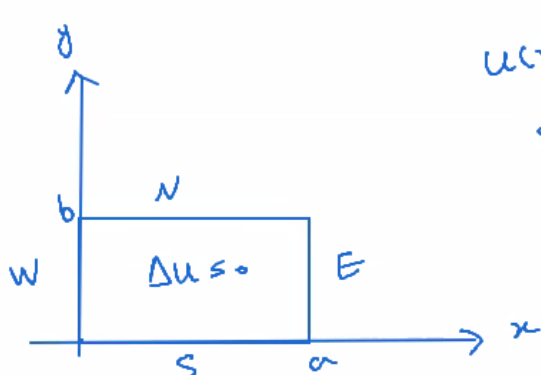
\includegraphics[width = 0.5 \textwidth]{1.png}
\end{center}

We use separation of variables such that $u(x,y) = X(x) Y(y)$, and substitute that and boundary conditions into $\Delta u = 0$. This gives us to problems -- One with $X(x)$ and $Y(y)$. We then superimpose the eigenfunctions and find the coefficients with inhomogeneous boundary conditions. 

Let's continue the polar coordinates example that we started last class. 

\section{Example 18}

$\Delta e = u_{rr} + \frac{1}{r} u_r + \frac{1}{r^2} u_{\theta \theta} = 0$, with a domain of $(r, \theta) \in \Omega$. We then have a boundary condition of $u(a, \theta) = f(\theta), \theta \in [0, 2 \pi]$. As $r \to 0$, $u(r,\theta) $ is bounded. 

\hfill

Solution: We use the method of separation of variables. 

$$u(r,\theta) = R(r) \Theta (\theta)$$

Substitute into $\Delta u = 0$:

$$- \left( \frac{r^2 R''}{R} + \frac{r R'}{R} \right) = \frac{\Theta''}{\Theta} = - \lambda$$

$\Theta$ function:

$$\Theta'' + \lambda \Theta = 0$$

$$\Theta(0) = \Theta(2 \pi)$$

$$\Theta'(0) = \Theta' (2 \pi)$$

Hence this is a P3 problem. As a result, eigenvalues are $\lambda_n = n^2$ and the eigenfunctions are $\Theta_n = \left\{ \cos (n \theta), \sin (n \theta) \right\} $


\hfill

Now for $R$:

when $n = 0$: $\Rightarrow \frac{r^2 R_0 ''}{R_0} + \frac{r R_0 '}{R_0} = 0 \Rightarrow \frac{\ud}{\ud r} (r R_0') = 0$. 

$R_0 = A \ln(r) + B$. Since $u$ is bounded as $r \to 0$. To be bounded, $A = 0$ and therefore $R_0 = B$. 

When $n \neq 0$, we get $r^2 R_n'' + r R_n' = n^2 R_n$. This is a Cauchy-Euler equation, and hence our guess solution is $R_n(r) = A_n r^k$. Substitute into out BVP and we get the following:

$$A_n k (k-1) r^{k-2} r^2 + A_n k r^{k-1} r = n^2 A_n r^k$$

$$\Rightarrow A_n r^k \left[ k^2 - k + k - n^2 \right] = 0 \Rightarrow k = \pm n$$

As a result, $R_n = A_n r^n + B_n r^{-n}$. 

Since $u$ is bounded as $r \to 0$, $B_n = 0$. 

Now let's superimpose the eigensolutions:

$$u(r, \theta) = C_0 + \sum_{n=1}^\infty \left[ C_n \cos (n \theta) + d_n \sin (n \theta) \right] r^n$$

Now, substitute the other boundary conditions to determine the coefficients. Apply the inhomogeneous boundary conditions: $r = a$

$$R(\theta) = u(r, \theta)= C_0 + \sum_{n=1}^\infty \left[ C_n \cos (n \theta) + d_n \sin(n \theta) \right] a^n$$

We need to write the Fourier series for $f(\theta)$. If we do this, we write:

$$f(\theta) = \frac{a_0}{2} + \sum_{n=1}^\infty \left[ a_n \cos (n \theta) = b_n \sin (n \theta) \right]$$

Matching coefficients we find that $c_0 = \frac{a_0}{2}$ and $c_n = a_n a^{-n}$ and $d_n = b_n a^{-n}$. 

Finally, the result is:

$$u(r, \theta) = \frac{a_0}{2} + \sum_{n=1}^\infty a^{-n} r^n \left( a_n \cos(n \theta) + b_n \sin(n \theta) \right) $$

\section{Boundary Conditions for Laplace Equations in Polar Coordinates}

\subsection*{Dirichlet Boundary Conditions}

$$\Theta(0) = \Theta(\alpha) = 0$$

where $\alpha$ is an angle.

This is a P1 problem, and hence $\lambda_n = \left( \frac{n \pi}{\alpha} \right)^2$ with $\Theta_n = \sin \left( \frac{n \pi}{\alpha} \theta \right)$ for $n \in \NN$

\begin{center}
    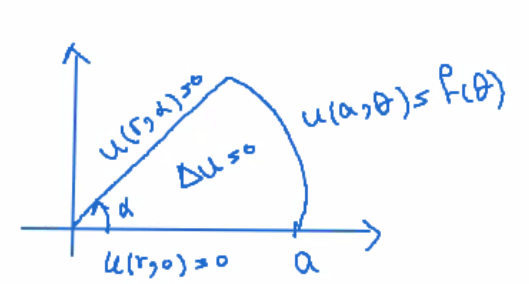
\includegraphics[width = 0.6 \textwidth]{2.png}
\end{center}

\subsection*{Neumann Boundary Conditions}

$$\Theta' (0) = \Theta' (\alpha) = 0$$

This is a P2 problem and hence:

$$n = 0, \quad \Theta_0 = 1$$

$$n \in \NN, \quad \lambda_n = \left( \frac{n \pi}{\alpha} \right)^2, \quad \Theta_n = \cos \left( \frac{n \pi}{\alpha} \theta \right)$$

\begin{center}
    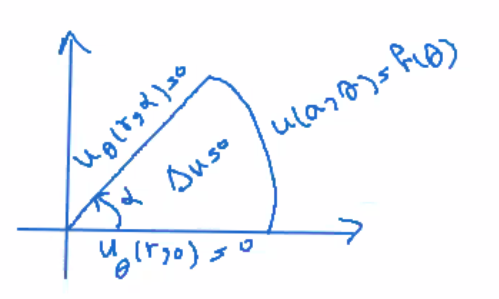
\includegraphics[width = 0.6 \textwidth]{3.png}
\end{center}

\subsection*{Periodic Boundary Conditions}

$$\Theta(0) = \Theta(2 \pi), \Theta'(0) = \Theta'(2 \pi)$$

P3 problem, and hence:

$\lambda_0 = 0 \to \Theta_0 = 1$

$$\lambda_n = \left( \frac{n \pi}{\pi} \right)^2 = n^2, \quad \Theta_n = \left\{ \cos(n \pi), \sin \left( n \pi \right) \right\} \text {for } n \in \NN$$

\subsection*{Mixed Boundary Conditions, Type 1}

$$\Theta(0) = \Theta'(\alpha) = 0 \Rightarrow \lambda_n = \left( \frac{(2n-1) \pi}{2 \alpha} \right)^2, \quad \Theta_n = \sin \left( \frac{(2n-1) \pi}{2 \alpha} \theta \right) \text { for } n \in \NN$$

\subsection*{Mixed Boundary Conditions, Type 2}

$$\Theta'(0) = \Theta(\alpha) \Rightarrow \lambda_n = \left( \frac{(2n-1) \pi}{2 \alpha} \right)^2, \quad \Theta_n = \cos \left( \frac{(2n-1) \pi}{2 \alpha} \theta \right) \text {for } n \in \NN$$

\section{Example 19}

$$\Delta u = 0, \quad r \in [0,1], \quad \theta \in (0, \alpha)$$

$$u(r,0) = 0, \quad u(r, \alpha) = 0, \quad r \in [0,1)$$

$$u(1, \theta) = 2 \theta, \quad \text { for } \theta \in (0, \alpha)$$

\begin{center}
    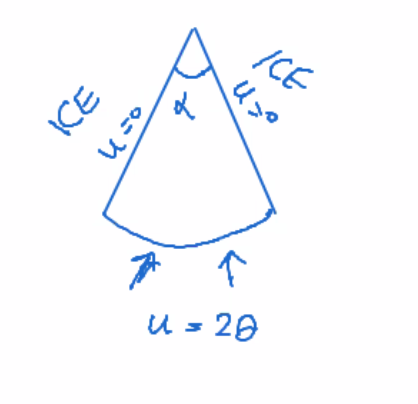
\includegraphics[width = 0.6 \textwidth]{4.png}
\end{center}

Solution: $u(r, \theta) = R(r) \Theta (\theta)$, similarly to example 18. 

$\Theta$ problem:

$$\Theta'' + \lambda \Theta = 0$$

$$\Theta(0) = \Theta(\alpha) = 0$$

Hence, $\lambda_n = \left( \frac{n \pi}{\alpha} \right)^2$ and $\Theta_n = \sin \left( \frac{n \pi}{\alpha} \theta \right), \quad \text{ for }n \in NN$

R-problem: 

$$r^2 R'' + r R' - ( \frac{n \pi}{\alpha})^2 R = 0$$

As this is a Cauchy-Euler equation, we get the following:

$$R_n(r) = A_n r^{\frac{n \pi}{\alpha}} + B_n r^{- \frac{n \pi}{\alpha}}$$

This is bounded as $r \to 0$ and hence $B_n = 0$. 

Hence:

$$u(r, \theta) = \sum_{n=1}^\infty C_n r^{\frac{n \pi}{\alpha}} \sin \left( \frac{n \pi}{\alpha} \theta \right)$$. 

What about $u(1, \theta)$?

$u(1, \theta) = 2 \theta$. Substituting these values, we get:

$$u(1, \theta) = 2 \theta = \sum_{n=1}^\infty C_n \sin \left( \frac{n \pi \theta}{\alpha} \right)$$

We need to write $2 \theta$ in a Fourier Sine Series. 

Hence, 

$$C_n = b_n = \frac{2}{\alpha} \int_0^\alpha 2 \theta \sin \left( \frac{n \pi \theta}{\alpha} \right) \ud \theta = \frac{-4 \theta}{\alpha} \frac{\alpha}{n \pi}  \left. \cos \left( \frac{n \pi \theta}{\alpha} \right) \right|_0^\alpha + \underbrace{ \frac{4}{n \pi} \int_0^\alpha \cos \left( \frac{n \pi }{\alpha} \theta \right) \ud \theta}_{ = 0}$$

$$ = \frac{4 \alpha}{n \pi} (-1)^{n+1}$$

Hence, 

$$u(r, \theta) = \sum_{n=1}^\infty \frac{4 \alpha}{n \pi} (-1)^{n+1} r^{\frac{n \pi}{\alpha}} \sin \left( \frac{n \pi \theta}{\alpha} \right)$$

\section{Example 20}

We start with the following conditions:

Condition 1:

$$u(r, - \pi) = u(r, \pi)$$

Condition 2:

$$u_{\theta} (r, - \pi) = u_{\theta} (r, \pi)$$

Hence, we have periodic boundary conditions. 

Condition 3:

$$u(\phi, \theta) = \sin(3 \theta), \quad \text{ for } \theta \in [-\pi, \pi]$$

Condition 4:

$$u(1, \theta) = \sin^2 (\theta), \quad \text{ for } \theta \in [-\pi, \pi]$$


\begin{center}
    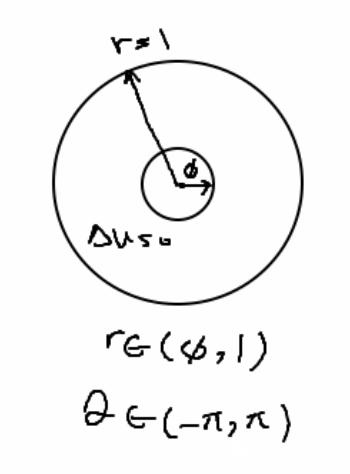
\includegraphics[width = 0.3 \textwidth]{6.png}
\end{center}


Similarly, we use separation of variables, similar to examples 18 and 19. 

For the $\Theta$ problem, we get a P3 boundary conditions and hence we have a solution of:

$\lambda_0 = 0 \to \Theta_0 = 0$

$$\lambda_n = n^2 \to \Theta_n = \cos(n \theta) \text{ or } \sin(n \theta)$$

For the R problem, we get:

$$R_n(r) = A_n r^n + B_n r^{-n}$$

Now, we have data at $r = \phi$ and $r = 1$. Therefore, we break the problem into $u(r, \theta) = u_{I} (r, \theta) + u_{O} (r, \theta)$ for inner and outer, respectively. 

$u_I$ satisfied conditions 1 and 3 $\to u_I (1, \theta) = 0$ and $u_I (\phi, \theta) = \sin(3 \theta)$

$u_0$ satisfies 1, 2, and 4, $\to u_0(\phi, \theta) = 0$ and $u_0 (1, \theta) = \sin^2 (\theta)$

$$R_{I,n}(1) = 0 \Rightarrow R_{I,n} = A_n (r^n - r^{-n})$$

$$u_I (r, \theta) = C_0 + \sum_{n=1}^\infty \left( C_n \cos (n \theta) + d_n \sin (n \theta) \right) R_{I,n}$$

Substituting boundary conditions:

$$u_{I}(\phi, \theta) = \sin(3 \theta) = C_0 + \sum_{n=1}^\infty \left( C_n \cos(n \theta) + d_n \sin(n \theta) \right) \left(\phi^n - \phi^{-n} \right)$$

Therefore, for any $n$, $C_n = 0$. For $d_n$ for $n \neq 3$, $d_n = 0$. However, $d_3 = \frac{1}{\phi^3 - \phi^{-3}}$

Therefore:

$$u_I(r, \theta) = \sin(3 \theta) \frac{r^3 - r^{-3}}{\phi^3 - \phi^{-3}}$$

Now let's do the same for the outer:

$$R_{O, n} (\phi) = 0 \Rightarrow R_{O,n} = B_n \left(r^2 - \phi^{2n} r^{-n} \right)$$

$$u_O (r, \theta) = a_n + \sum_{n=1}^\infty (a_n \cos (n \theta) + b_n \sin(n \theta)) R_{O, n} (r)$$

Now, let's substitute inhomogeneous boundary conditons:

$$u_o (1, \theta) = \sin^2  (\theta) = a_0 + \sum_{n=1}^\infty \left[ a_n \cos(n \theta) + b_n \sin(n \theta) \right] (1 - \phi^{2n})$$

We need to use a trigonometric identity:

$$\sin^2  (\theta) = \frac{1}{2} \left(1 - cos (2 \theta) \right)$$

Therefore, 

$$\frac{1}{2} \left(1 - cos (2 \theta) \right) =  a_0 + \sum_{n=1}^\infty \left[ a_n \cos(n \theta) + b_n \sin(n \theta) \right] (1 - \phi^{2n})$$

$$\Rightarrow a_0 = \frac{1}{2}, \quad a_2 = \frac{1}{2 (1 - \phi^{2n})}, \quad a_{n \neq 2} = 0, \quad b_n = 0$$

$$\Rightarrow u_0 (r, \theta) = \frac{1}{2} \left( 1 - \frac{r^2 - \phi^4 r^{-2}}{1 - \phi^4} \cos(2 \theta) \right)$$

Finally, $u(r, \theta) = u_I (r, \theta) + u_o (r, \theta)$

\section{Example 21}

A wedge with insulating boundary conditions on $\theta = 0$ and $\theta = \alpha < 2 \pi$. 

$\Delta u = 0$, $u_\theta (r,0) = 0$ and $u_\theta (r, \alpha) = 0$. 

$u(a, \theta) = f(\theta)$

\begin{center}
    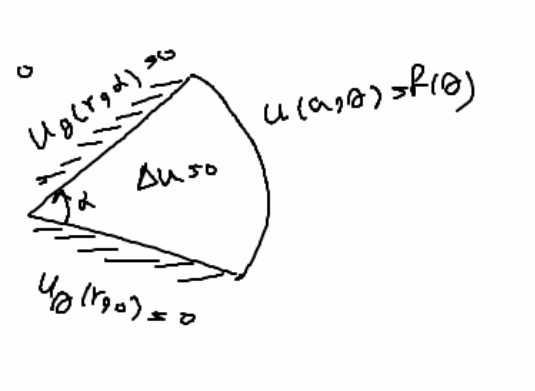
\includegraphics[width = 0.4 \textwidth]{8.png}
\end{center}

Using separation of variables, 

$$- \left( \frac{r^2 R''}{R} + \frac{r R'}{R} \right) = \frac{\Theta''}{\Theta} = - \lambda$$

Theta problem: P2

$$\lambda_0 = 0, \quad \Theta_0 = 0$$

$$\lambda_n = \left( \frac{n \pi}{\alpha} \right)^2 \to \Theta_n = \cos \left( \frac{n \pi}{\alpha} \theta \right)$$

R problem:

$$r^2 R_n'' + r R_n' - n^2 R_n = 0$$



%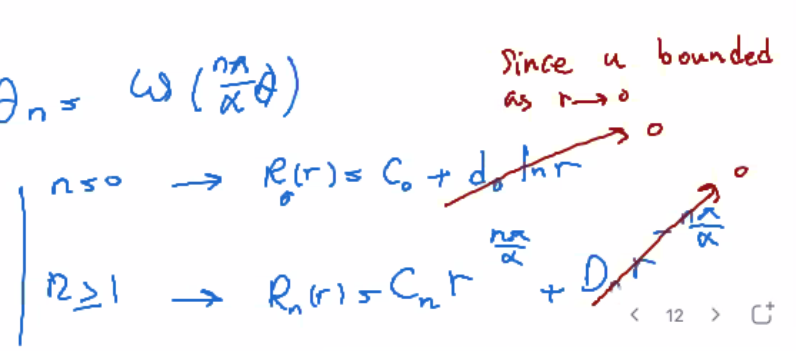
\includegraphics[width = 0.4 \textwidth]{11.png}


$$n = 0 \to R_0(r) + C_0 + \underbrace{d_0 \ln(r)}_{ = 0}$$

$$n \geq 1 \to R_n(r) = C_n r^{\frac{n \pi}{\alpha}} + \underbrace{D_n r^{- \frac{n \pi}{\alpha}}}_{ = 0}$$

The portions that equal zero equal zero because $u$ is bounded as $r \to 0$. 


%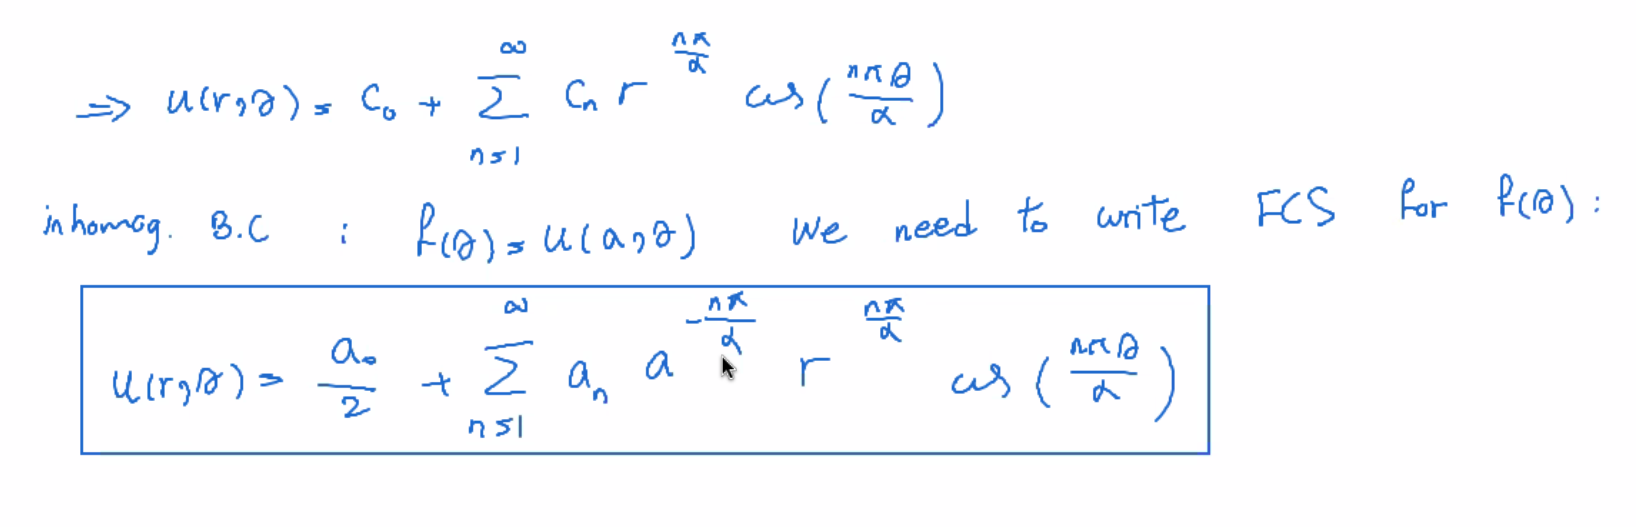
\includegraphics[width = 0.8 \textwidth]{10.png}


$$\Rightarrow u(r, \theta) = C_0 + \sum_{n=1}^\infty C_n r^{\frac{n \pi}{\alpha}} \cos \left( \frac{n \pi \theta}{\alpha} \right)$$

Inhomogeneous boundary conditions: $f(\theta) = u(a, \theta)$. We need to write the Fourier cosine series for $f(\theta)$:

$$u(r, \theta) = \frac{a_0}{2} + \sum_{n=1}^\infty a_n a^{- \frac{n \pi}{\alpha}} r^{\frac{n \pi}{\alpha}} \cos \left( \frac{n \pi \theta}{\alpha} \right)$$






\end{document}